% !TEX root = tnnls_relation_gait.tex

\ifx\allfiles\undefined
    % !TEX root = tnnls_relation_gait.tex

%% bare_jrnl.tex
%% V1.4b
%% 2015/08/26
%% by Michael Shell
%% see http://www.michaelshell.org/
%% for current contact information.
%%
%% This is a skeleton file demonstrating the use of IEEEtran.cls
%% (requires IEEEtran.cls version 1.8b or later) with an IEEE
%% journal paper.
%%
%% Support sites:
%% http://www.michaelshell.org/tex/ieeetran/
%% http://www.ctan.org/pkg/ieeetran
%% and
%% http://www.ieee.org/

%%*************************************************************************
%% Legal Notice:
%% This code is offered as-is without any warranty either expressed or
%% implied; without even the implied warranty of MERCHANTABILITY or
%% FITNESS FOR A PARTICULAR PURPOSE!
%% User assumes all risk.
%% In no event shall the IEEE or any contributor to this code be liable for
%% any damages or losses, including, but not limited to, incidental,
%% consequential, or any other damages, resulting from the use or misuse
%% of any information contained here.
%%
%% All comments are the opinions of their respective authors and are not
%% necessarily endorsed by the IEEE.
%%
%% This work is distributed under the LaTeX Project Public License (LPPL)
%% ( http://www.latex-project.org/ ) version 1.3, and may be freely used,
%% distributed and modified. A copy of the LPPL, version 1.3, is included
%% in the base LaTeX documentation of all distributions of LaTeX released
%% 2003/12/01 or later.
%% Retain all contribution notices and credits.
%% ** Modified files should be clearly indicated as such, including  **
%% ** renaming them and changing author support contact information. **
%%*************************************************************************


% *** Authors should verify (and, if needed, correct) their LaTeX system  ***
% *** with the testflow diagnostic prior to trusting their LaTeX platform ***
% *** with production work. The IEEE's font choices and paper sizes can   ***
% *** trigger bugs that do not appear when using other class files.       ***                          ***
% The testflow support page is at:
% http://www.michaelshell.org/tex/testflow/

\documentclass[journal]{IEEEtran}
%
% If IEEEtran.cls has not been installed into the LaTeX system files,
% manually specify the path to it like:
% \documentclass[journal]{../sty/IEEEtran}

% Some very useful LaTeX packages include:
% (uncomment the ones you want to load)

% *** MISC UTILITY PACKAGES ***
%
%\usepackage{ifpdf}
% Heiko Oberdiek's ifpdf.sty is very useful if you need conditional
% compilation based on whether the output is pdf or dvi.
% usage:
% \ifpdf
%   % pdf code
% \else
%   % dvi code
% \fi
% The latest version of ifpdf.sty can be obtained from:
% http://www.ctan.org/pkg/ifpdf
% Also, note that IEEEtran.cls V1.7 and later provides a builtin
% \ifCLASSINFOpdf conditional that works the same way.
% When switching from latex to pdflatex and vice-versa, the compiler may
% have to be run twice to clear warning/error messages.

% *** CITATION PACKAGES ***

\usepackage{tabularx}
\usepackage{longtable}
\usepackage{threeparttable}
\usepackage{cite}

% cite.sty was written by Donald Arseneau
% V1.6 and later of IEEEtran pre-defines the format of the cite.sty package
% \cite{} output to follow that of the IEEE. Loading the cite package will
% result in citation numbers being automatically sorted and properly
% "compressed/ranged". e.g., [1], [9], [2], [7], [5], [6] without using
% cite.sty will become [1], [2], [5]--[7], [9] using cite.sty. cite.sty's
% \cite will automatically add leading space, if needed. Use cite.sty's
% noadjust option (cite.sty V3.8 and later) if you want to turn this off
% such as if a citation ever needs to be enclosed in parenthesis.
% cite.sty is already installed on most LaTeX systems. Be sure and use
% version 5.0 (2009-03-20) and later if using hyperref.sty.
% The latest version can be obtained at:
% http://www.ctan.org/pkg/cite
% The documentation is contained in the cite.sty file itself.

% *** GRAPHICS RELATED PACKAGES ***
%
\usepackage[pdftex]{graphicx}
\usepackage{rotating}
\ifCLASSINFOpdf
  % \usepackage[pdftex]{graphicx}
  % declare the path(s) where your graphic files are
  % \graphicspath{{../pdf/}{../jpeg/}}
  % and their extensions so you won't have to specify these with
  % every instance of \includegraphics
  % \DeclareGraphicsExtensions{.pdf,.jpeg,.png}
\else
  % or other class option (dvipsone, dvipdf, if not using dvips). graphicx
  % will default to the driver specified in the system graphics.cfg if no
  % driver is specified.
  % \usepackage[dvips]{graphicx}
  % declare the path(s) where your graphic files are
  % \graphicspath{{../eps/}}
  % and their extensions so you won't have to specify these with
  % every instance of \includegraphics
  % \DeclareGraphicsExtensions{.eps}
\fi
% graphicx was written by David Carlisle and Sebastian Rahtz. It is
% required if you want graphics, photos, etc. graphicx.sty is already
% installed on most LaTeX systems. The latest version and documentation
% can be obtained at:
% http://www.ctan.org/pkg/graphicx
% Another good source of documentation is "Using Imported Graphics in
% LaTeX2e" by Keith Reckdahl which can be found at:
% http://www.ctan.org/pkg/epslatex
%
% latex, and pdflatex in dvi mode, support graphics in encapsulated
% postscript (.eps) format. pdflatex in pdf mode supports graphics
% in .pdf, .jpeg, .png and .mps (metapost) formats. Users should ensure
% that all non-photo figures use a vector format (.eps, .pdf, .mps) and
% not a bitmapped formats (.jpeg, .png). The IEEE frowns on bitmapped formats
% which can result in "jaggedy"/blurry rendering of lines and letters as
% well as large increases in file sizes.
%
% You can find documentation about the pdfTeX application at:
% http://www.tug.org/applications/pdftex

% *** MATH PACKAGES ***
%
\usepackage{amsmath}
% A popular package from the American Mathematical Society that provides
% many useful and powerful commands for dealing with mathematics.
%
% Note that the amsmath package sets \interdisplaylinepenalty to 10000
% thus preventing page breaks from occurring within multiline equations. Use:
%\interdisplaylinepenalty=2500
% after loading amsmath to restore such page breaks as IEEEtran.cls normally
% does. amsmath.sty is already installed on most LaTeX systems. The latest
% version and documentation can be obtained at:
% http://www.ctan.org/pkg/amsmath

% *** SPECIALIZED LIST PACKAGES ***
%
\usepackage{algorithmic}
% algorithmic.sty was written by Peter Williams and Rogerio Brito.
% This package provides an algorithmic environment fo describing algorithms.
% You can use the algorithmic environment in-text or within a figure
% environment to provide for a floating algorithm. Do NOT use the algorithm
% floating environment provided by algorithm.sty (by the same authors) or
% algorithm2e.sty (by Christophe Fiorio) as the IEEE does not use dedicated
% algorithm float types and packages that provide these will not provide
% correct IEEE style captions. The latest version and documentation of
% algorithmic.sty can be obtained at:
% http://www.ctan.org/pkg/algorithms
% Also of interest may be the (relatively newer and more customizable)
% algorithmicx.sty package by Szasz Janos:
% http://www.ctan.org/pkg/algorithmicx

% *** ALIGNMENT PACKAGES ***
%
\usepackage{array}
% Frank Mittelbach's and David Carlisle's array.sty patches and improves
% the standard LaTeX2e array and tabular environments to provide better
% appearance and additional user controls. As the default LaTeX2e table
% generation code is lacking to the point of almost being broken with
% respect to the quality of the end results, all users are strongly
% advised to use an enhanced (at the very least that provided by array.sty)
% set of table tools. array.sty is already installed on most systems. The
% latest version and documentation can be obtained at:
% http://www.ctan.org/pkg/array

% IEEEtran contains the IEEEeqnarray family of commands that can be used to
% generate multiline equations as well as matrices, tables, etc., of high
% quality.

% *** SUBFIGURE PACKAGES ***
\usepackage[caption=false,font=footnotesize]{subfig}
%\ifCLASSOPTIONcompsoc
%  \usepackage[caption=false,font=normalsize,labelfont=sf,textfont=sf]{subfig}
%\else
%  \usepackage[caption=false,font=footnotesize]{subfig}
%\fi
% subfig.sty, written by Steven Douglas Cochran, is the modern replacement
% for subfigure.sty, the latter of which is no longer maintained and is
% incompatible with some LaTeX packages including fixltx2e. However,
% subfig.sty requires and automatically loads Axel Sommerfeldt's caption.sty
% which will override IEEEtran.cls' handling of captions and this will result
% in non-IEEE style figure/table captions. To prevent this problem, be sure
% and invoke subfig.sty's "caption=false" package option (available since
% subfig.sty version 1.3, 2005/06/28) as this is will preserve IEEEtran.cls
% handling of captions.
% Note that the Computer Society format requires a larger sans serif font
% than the serif footnote size font used in traditional IEEE formatting
% and thus the need to invoke different subfig.sty package options depending
% on whether compsoc mode has been enabled.
%
% The latest version and documentation of subfig.sty can be obtained at:
% http://www.ctan.org/pkg/subfig

% *** FLOAT PACKAGES ***
%
%\usepackage{fixltx2e}
% fixltx2e, the successor to the earlier fix2col.sty, was written by
% Frank Mittelbach and David Carlisle. This package corrects a few problems
% in the LaTeX2e kernel, the most notable of which is that in current
% LaTeX2e releases, the ordering of single and double column floats is not
% guaranteed to be preserved. Thus, an unpatched LaTeX2e can allow a
% single column figure to be placed prior to an earlier double column
% figure.
% Be aware that LaTeX2e kernels dated 2015 and later have fixltx2e.sty's
% corrections already built into the system in which case a warning will
% be issued if an attempt is made to load fixltx2e.sty as it is no longer
% needed.
% The latest version and documentation can be found at:
% http://www.ctan.org/pkg/fixltx2e

%\usepackage{stfloats}
% stfloats.sty was written by Sigitas Tolusis. This package gives LaTeX2e
% the ability to do double column floats at the bottom of the page as well
% as the top. (e.g., "\begin{figure*}[!b]" is not normally possible in
% LaTeX2e). It also provides a command:
%\fnbelowfloat
% to enable the placement of footnotes below bottom floats (the standard
% LaTeX2e kernel puts them above bottom floats). This is an invasive package
% which rewrites many portions of the LaTeX2e float routines. It may not work
% with other packages that modify the LaTeX2e float routines. The latest
% version and documentation can be obtained at:
% http://www.ctan.org/pkg/stfloats
% Do not use the stfloats baselinefloat ability as the IEEE does not allow
% \baselineskip to stretch. Authors submitting work to the IEEE should note
% that the IEEE rarely uses double column equations and that authors should try
% to avoid such use. Do not be tempted to use the cuted.sty or midfloat.sty
% packages (also by Sigitas Tolusis) as the IEEE does not format its papers in
% such ways.
% Do not attempt to use stfloats with fixltx2e as they are incompatible.
% Instead, use Morten Hogholm'a dblfloatfix which combines the features
% of both fixltx2e and stfloats:
%
% \usepackage{dblfloatfix}
% The latest version can be found at:
% http://www.ctan.org/pkg/dblfloatfix

%\ifCLASSOPTIONcaptionsoff
%  \usepackage[nomarkers]{endfloat}
% \let\MYoriglatexcaption\caption
% \renewcommand{\caption}[2][\relax]{\MYoriglatexcaption[#2]{#2}}
%\fi
% endfloat.sty was written by James Darrell McCauley, Jeff Goldberg and
% Axel Sommerfeldt. This package may be useful when used in conjunction with
% IEEEtran.cls'  captionsoff option. Some IEEE journals/societies require that
% submissions have lists of figures/tables at the end of the paper and that
% figures/tables without any captions are placed on a page by themselves at
% the end of the document. If needed, the draftcls IEEEtran class option or
% \CLASSINPUTbaselinestretch interface can be used to increase the line
% spacing as well. Be sure and use the nomarkers option of endfloat to
% prevent endfloat from "marking" where the figures would have been placed
% in the text. The two hack lines of code above are a slight modification of
% that suggested by in the endfloat docs (section 8.4.1) to ensure that
% the full captions always appear in the list of figures/tables - even if
% the user used the short optional argument of \caption[]{}.
% IEEE papers do not typically make use of \caption[]'s optional argument,
% so this should not be an issue. A similar trick can be used to disable
% captions of packages such as subfig.sty that lack options to turn off
% the subcaptions:
% For subfig.sty:
% \let\MYorigsubfloat\subfloat
% \renewcommand{\subfloat}[2][\relax]{\MYorigsubfloat[]{#2}}
% However, the above trick will not work if both optional arguments of
% the \subfloat command are used. Furthermore, there needs to be a
% description of each subfigure *somewhere* and endfloat does not add
% subfigure captions to its list of figures. Thus, the best approach is to
% avoid the use of subfigure captions (many IEEE journals avoid them anyway)
% and instead reference/explain all the subfigures within the main caption.
% The latest version of endfloat.sty and its documentation can obtained at:
% http://www.ctan.org/pkg/endfloat
%
% The IEEEtran \ifCLASSOPTIONcaptionsoff conditional can also be used
% later in the document, say, to conditionally put the References on a
% page by themselves.

% *** PDF, URL AND HYPERLINK PACKAGES ***
%
\usepackage{url}
% url.sty was written by Donald Arseneau. It provides better support for
% handling and breaking URLs. url.sty is already installed on most LaTeX
% systems. The latest version and documentation can be obtained at:
% http://www.ctan.org/pkg/url
% Basically, \url{my_url_here}.

% *** Do not adjust lengths that control margins, column widths, etc. ***
% *** Do not use packages that alter fonts (such as pslatex).         ***
% There should be no need to do such things with IEEEtran.cls V1.6 and later.
% (Unless specifically asked to do so by the journal or conference you plan
% to submit to, of course. )

% correct bad hyphenation here
% \hyphenation{op-tical net-works semi-conduc-tor}
\usepackage{enumerate}
\usepackage{multirow}
\usepackage{color}
\usepackage{threeparttable}
\usepackage{booktabs}
\newcommand{\minus}{\scalebox{0.75}[1.0]{$-$}}
\newcommand{\bftab}[1]{{\fontseries{b}\selectfont#1}}
\newcommand{\tabincell}[2]{\begin{tabular}{@{}#1@{}}#2\end{tabular}}
\newcommand{\etal}{\textit{et al}.}
\newcommand{\ie}{\textit{i.e.}}
\newcommand{\eg}{\textit{e.g.}}
\newcommand{\wrt}{\textit{w.r.t.}}
\newcommand{\vs}{\textit{vs.}}


\begin{document}
%
% paper title
% Titles are generally capitalized except for words such as a, an, and, as,
% at, but, by, for, in, nor, of, on, or, the, to and up, which are usually
% not capitalized unless they are the first or last word of the title.
% Linebreaks \\ can be used within to get better formatting as desired.
% Do not put math or special symbols in the title.
%\title{The Application and Research of Multi-modal Data in Auxiliary Diagnosis of Depression: A Survey
%}
\title{ Auxiliary Diagnosis of Depression Based on Multi-modal Data: A Survey
}
%%
%%
%% author names and IEEE memberships
%% note positions of commas and nonbreaking spaces ( ~ ) LaTeX will not break
%% a structure at a ~ so this keeps an author's name from being broken across
%% two lines.
%% use \thanks{} to gain access to the first footnote area
%% a separate \thanks must be used for each paragraph as LaTeX2e's \thanks
%% was not built to handle multiple paragraphs
%%
%
%\author{Saihui~Hou,
%	Xu~Liu,
%	Chunshui~Cao,
%	and~Yongzhen~Huang$^*$% <-this % stops a space
%	\thanks{$^*$ indicates the corresponding author.}% <-this % stops a space
%    \thanks{Saihui Hou and Yongzhen Huang is with School of Artificial Intelligence, Beijing Normal University, Beijing 100875, China. (Email: housaihui@bnu.edu.cn, huangyongzhen@bnu.edu.cn)}
%	\thanks{Xu Liu and Chunshui Cao are with Watrix Technology Limited Co. Ltd, Beijing 100088, China. (Email: xu.liu@watrix.ai, chunshuicao@watrix.ai)}
%    \thanks{This work is partially supported by the Fundamental Research Funds for the Central Universities.}
%    % \thanks{E-mail: housaihui@bnu.edu.cn, xu.liu@watrix.ai, chunshuicao@watrix.ai, huangyongzhen@bnu.edu.cn}
%	% \thanks{Manuscript received April 19, 2005; revised August 26, 2015.}
%}
%
%% note the % following the last \IEEEmembership and also \thanks -
%% these prevent an unwanted space from occurring between the last author name
%% and the end of the author line. i.e., if you had this:
%%
%% \author{....lastname \thanks{...} \thanks{...} }
%%                     ^------------^------------^----Do not want these spaces!
%%
%% a space would be appended to the last name and could cause every name on that
%% line to be shifted left slightly. This is one of those "LaTeX things". For
%% instance, "\textbf{A} \textbf{B}" will typeset as "A B" not "AB". To get
%% "AB" then you have to do: "\textbf{A}\textbf{B}"
%% \thanks is no different in this regard, so shield the last } of each \thanks
%% that ends a line with a % and do not let a space in before the next \thanks.
%% Spaces after \IEEEmembership other than the last one are OK (and needed) as
%% you are supposed to have spaces between the names. For what it is worth,
%% this is a minor point as most people would not even notice if the said evil
%% space somehow managed to creep in.
%
%% The paper headers
%\markboth{IEEE Transactions on Neural Networks and Learning Systems}%
%{Saihui Hou \MakeLowercase{\textit{et al.}}: GQAN: Towards the Interpretability of Silhouette-based Gait Recognition}
%% The only time the second header will appear is for the odd numbered pages
%% after the title page when using the twoside option.
%%
%% *** Note that you probably will NOT want to include the author's ***
%% *** name in the headers of peer review papers.                   ***
%% You can use \ifCLASSOPTIONpeerreview for conditional compilation here if
%% you desire.
%
%% If you want to put a publisher's ID mark on the page you can do it like
%% this:
%%\IEEEpubid{0000--0000/00\$00.00~\copyright~2015 IEEE}
%% Remember, if you use this you must call \IEEEpubidadjcol in the second
%% column for its text to clear the IEEEpubid mark.
%
%% use for special paper notices
%%\IEEEspecialpapernotice{(Invited Paper)}
%
%% make the title area
\maketitle

\fi

\section{Depression recognition method based on Brain Imaging}
\label{sec_approach}
Compared with healthy people, the brain structure and function of patients with depression may have some abnormalities~\cite{2018Neural}, which will inhibit the patient's thinking speed. In severe cases, it will lead to cognitive impairment and even a state of mental illness.
In addition, depression can atrophy the hippocampus of the patient's brain, alter neurotransmitters in the brain, and cause chronic inflammation, resulting in memory loss and frequent fatigue, which greatly reduces the patient's energy level and motivation, making it difficult for the patient to socialize.
These findings found a new breakthrough point for the study of the pathogenesis of depression. With the development of neuroimaging technology, great progress has been made in the exploration of neurobiological mechanisms of depression.

Brain structure imaging studies mainly focus on the frontal lobe, temporal lobe, amygdala, basal ganglia, cingulate gyrus, hippocampus and other brain regions of the cerebral cortex.
Depression research based on brain imaging data is mainly divided into brain structure, brain function and brain metabolic imaging.
Brain function imaging studies of depression mainly include Functional Nearinfrared Spectroscopy (fNIRS), nuclear Magnetic Resonance Imaging (MRI), etc. Brain metabolic imaging studies to explore depression mainly include Positron Emission computed Tomography (PET) and Magnetic Resonance Spectroscopy (MRS), etc.

As shown in Fig \ref{brain-imaging}, brain images are acquired by scanning the subject's brain with various precision instruments, and there are significant differences in brain volume and structure among different people, as well as a large amount of interference and noise in the acquisition data due to the slight head movement of the subject or the scanning equipment during the acquisition process, so image pre-processing is needed to eliminate individual differences and noise interference. Among them, image normalization includes head movement correction, brain tissue separation, and segmentation alignment, this step can remove individual differences and head movement interference. Image denoising is mainly used to remove the noise generated by the external environment and equipment, and the common methods include Gaussian filtering, band-pass filtering, wavelet transform, etc. In the feature extraction process, linear models, wavelet packet decomposition and other methods are usually applied to extract time and frequency domain features, or the features of each brain region are extracted according to standard brain templates, and then redundant and irrelevant features are removed using feature selection algorithms, and the effective features are fused for subsequent classification.

\begin{figure}[tbp]
	\centering	
	\label{fig_hard_case1}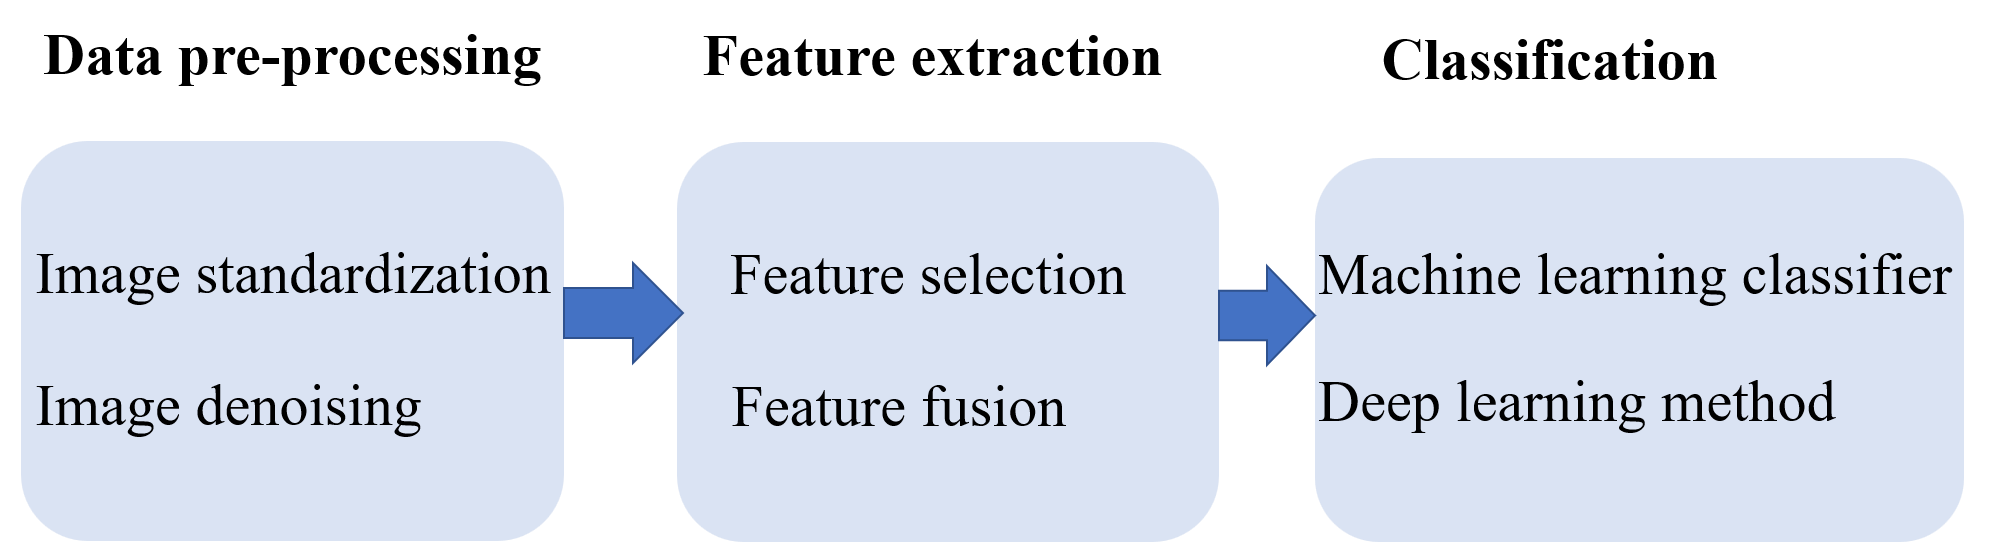
\includegraphics[width=0.8\linewidth]{figures/depression/brain-imaging.png}		
	\caption{
	Flow diagram of depression detection based on brain imaging.
	}
	\label{brain-imaging}
\end{figure}

\subsection{fNIRS}
\label{sec_fquality}
%%%%%%%%%%%%%%%%%%%%%%%%%%%%%%%%%%%%%%%
fNIRS utilizes the scattering properties of blood to near-infrared light to obtain changes in oxyhemoglobin and deoxyhemoglobin during brain activity.
It is an important tool for the study of brain function imaging. It can be used to compare the differences in brain function between healthy and mentally ill patients, and to achieve non-invasive detection of brain function~\cite{2018Reduced,2019Brain,2014Relationship,2016Correlation,2019The}.

In recent years, machine learning techniques have shown great potential in the diagnosis and treatment of mental health disorders including depression~\cite{2019Machine}~\cite{2017Machine}. 
The most common machine learning algorithms for predictive classification such as Support Vector Machines (SVM), Decision Trees (DT) and naïve bayes,etc, have been applied to fNIRS data to classify Major Depressive Disorder (MDD) patients and healthy individuals. All of these methods have yielded good results in depression identification~\cite{2017Automatic}. 
Hong et al.~\cite{2015Automatic} designed a SVM based classifier to classify the features extracted from fNIRS.
There are also some integrated machine learning methods that have been applied in depression recognition, such as Random Forest (RF) and Extreme Gradient Boosting (XGBoost),etc. Zhu et al.~\cite{2020Classifying} extracted ten features from HbO signals, from each channel served as inputs to XGBoost and RF algorithms developed for each block and combination of successive blocks.

%Fu recruited 43 patients with bipolar depression to assess changes in frontal region oxyhemoglobin (oxy-Hb) levels during the TOL task and VFT using a 41-channel NIRS system. The results showed that the level of oxyhemoglobin in the prefrontal cortex was significantly lower in patients with bipolar depression~\cite{2018Reduced}.
%By studying the association between brain mitochondrial dysfunction and mood disorders, Holper~\cite{2019Brain} found that brain cytochrome cyclooxygenase (COX) activity was decreased in patients with depression, and was inversely proportional to the severity of depression.
%Liu confirmed that hypoactivation in prefrontal cortex of MDD patients with anxious and obsessive-compulsive symptoms~\cite{2014Relationship}.
%Kawano found that oxy-Hb in the frontal lobe was negatively correlated with depression detection scale scores on NIRS~\cite{2016Correlation}.

Traditional machine learning classification methods require a priori feature preprocessing to train the model, extensive reliance on manual feature extraction and selection. By using deep Learning methods like Artificial Neural Network (ANN), Deep Neural Networks (DNNs) and Long Short-Term Memory (LSTM), etc, records can be fed directly to the algorithm for training, avoiding the need for feature selection. As a result, more and more researchers have applied deep learning algorithms to multimodal fNIRS classification tasks~\cite{2022Deep},and have also achieved high accuracy in depression recognition and diagnosis~\cite{2021Depression}.
Ma et al.\cite{2020DISTINGUISHING} was able to distinguish bipolar depression from major depressive disorder in adults during a verbal fluency task by using an LSTM~.
Chao et al.~\cite{2021fNIRS} used a cascade forward neural network to classify depression and achieved excellent results.


\begin{figure}[tbp]
	\centering
	\subfloat[Data Collection]{
		\label{fig_hard_case1}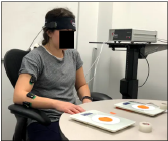
\includegraphics[width=0.5\linewidth]{figures/depression/fNIRS3.png}
	}
	%\\
	%\vspace{-2mm}
	\subfloat[fNIRS]{
		\label{fig_hard_case2}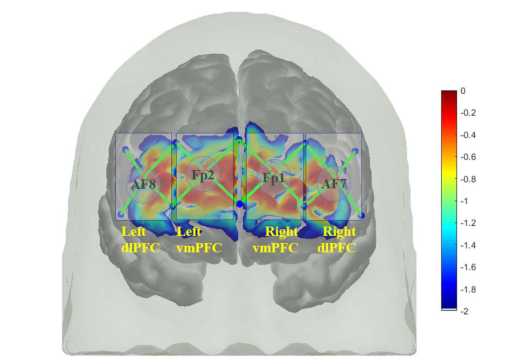
\includegraphics[width=0.5\linewidth]{figures/depression/fNIRS4.png}
	}
	
	\caption{
    Participant instrumented and sitting upright.
    PFC activation sensitivity map of fNIRS probe. Red and blue dots indicate sources and detectors, respectively , green lines indicate channels. Source-detector separation distance is 2.5 cm~\cite{2020Classifying}.
	}
	\label{fNIRS}
\end{figure}

\subsection{MRI}
%\label{sec_fquality}
%%%%%%%%%%%%%%%%%%%%%%%%%%%%%%%%%%%%%%%

MRI is a new examination technology based on the principle that atomic nuclei with magnetic distance can produce transitions between energy levels under the action of a magnetic field. It helps to check the energy state and cerebral blood flow of the patient's brain.
In MRI techniques, the MRI images obtained with different scanning parameters include structural MRI (sMRI) and functional MRI (fMRI).

%A meta-analysis of 29 studies fulfilling specific criteria was performed, Santos ecreased hippocampal volume found widespread in patients with major depressive disorder~\cite{Santos2018Global}.Narita found that the volume of the ventral prefrontal cortex decreased in patients with depression~\cite{2011Volume}.
%Taki examined structural differences in regional gray matter volume between depressed patients and non-depressed normal subjects by voxel-based morphometry (VBM) based on  MRI, found bilateral medial frontal lobes in depressed patients and significantly smaller volume in the right central front~\cite{2005Male}.
%Zhang investigated the relationship between subthreshold depression (StD) and MDD, and found similar patterns of gray matter volume(GMV) reduction in the orbitofrontal cortex and left temporal gyrus~\cite{2020Subthreshold}.
%In addition, other studies have found that different levels of depression are associated with changes in habenula volume~\cite{2013Habenula}~\cite{J2013P}.

\subsubsection{sMRI}
%\textbf{sMRI}
%%%%%%%%%%%%%%%%%%%%%%%%%%%%%%%%%%%%%%%%%%%%%%%%%%%%%%
The sMRI images can clearly show the anatomical structure of the brain with high spatial resolution and can be used to objectively reflect the structural morphological changes within the brain.
The detection of depression from sMRI scans usually includes processes such as image acquisition and preprocessing, feature extraction and selection, and classification. Machine learning methods have also been widely used, such as One Rule (OneR), SVM, Information Gain (IG) and ReliefF, etc~\cite{2013Evaluation}~\cite{P2020Radiological}.
Deep learning methods have brought out remarkable results in medical imaging analysis, such as Mousavian et al.~\cite{2019Depression} found that the pre-trained VGG 16 and fine- tuning produced good results.

\subsubsection{fMRI}
%\label{sec_fquality}
%%%%%%%%%%%%%%%%%%%%%%%%%%%%%%%%%%%%%%%
fMRI uses magnetic resonance imaging to measure changes in hemodynamics caused by neuronal activity. It can observe the changes of the brain through the small changes in the magnetic resonance signal caused by the oxygenation state of the brain, thereby revealing the relationship between brain activity and thinking. According to different experimental conditions, fMRI is mainly divided into Resting State fMRI (RS-fMRI) and Task State fMRI (TS-fMRI).

RS-fMRI collects data when the subjects are in a relaxed state. Since there is no task interference, it can help doctors understand brain development, diseases, etc~\cite{2018Disrupted}. RS-fMRI is mainly aimed at the analysis of regional brain activity and functional connectivity of brain regions.
Many researchers have built machine learning classification models to predict the accuracy of depression~\cite{2013Identifying,2019Intrinsic,2019Resting}.
Zeng et al.~\cite{2014Unsupervised} built an unsupervised machine learning model for MDD.
Bhaumik et al.~\cite{2016Multivariate} extracted the features of the left posterior cingulate cortex and the right dorsolateral prefrontal cortex and input it to the SVM classifier for depression recognition.
Yan et al.~\cite{2020Quantitative} exploited the hidden information embedded in dynamic functional connectivity (DFC) and developed an accurate and objective image-based diagnosis system for MDD.
To improve the generalization ability of classifiers, multicenter studies~\cite{2020Generalizable} have been conducted and cover deep learning algorithms.
Zhao et al.~\cite{2020Functional} established a generative adversarial network depression classification model based on functional brain network connections in a multicenter sample. Jun rt al.~\cite{2020Identifying} distinguished drug-naïve MDD patients from healthy controls using Graph Convolutional Networks (GCNs). 

TS-fMRI refers to the process of collecting data, subjects need to perform specific tasks, such as exercise, cognitive activities.
%Murrough utilized functional magnetic resonance imaging (fMRI) and two separate emotion perception tasks to examine the neural effects of ketamine in patients with treatment-resistant major depressive disorder(TRD), found that TRD patients had reduced neural responses to frontal faces in the right caudate nucleus compared to healthy volunteers~\cite{2015Regulation}.
%Johnston described an instrumental loss-avoidance and win-gain reinforcement learning functional magnetic resonance imaging study with 40 patients with highly treatment-resistant major depressive disorder and never-depressed controls, found that the predictive diagnostic accuracy of patients with abnormal striatal activity was as high as 97\%, while the predictive diagnostic accuracy of abnormal hippocampal activity was 84\%~\cite{2015Failure}.
Current research combining machine learning with TS fMRI is mainly related to emotional face stimulation, speech and music listening tasks, and this method enables individual-level analysis and reduces subjective misjudgments.
Machine learning classifiers have achieved good results in related research, such as Gaussian Process Classifiers(GPC), RF, SVM, etc~\cite{2013What}~\cite{2015Toward}.
Because deep learning has the advantages of reducing human intervention, deep analysis and feature extraction, selection and classification in the same optimal deep structure. Gui trained a Deep Learning Network (DLN) model with fMRI data of listening to positive and negative music~\cite{2019The1}.


\begin{figure}[tbp]
\centering
	\subfloat[sMRI images]{
		\label{fig_hard_case1}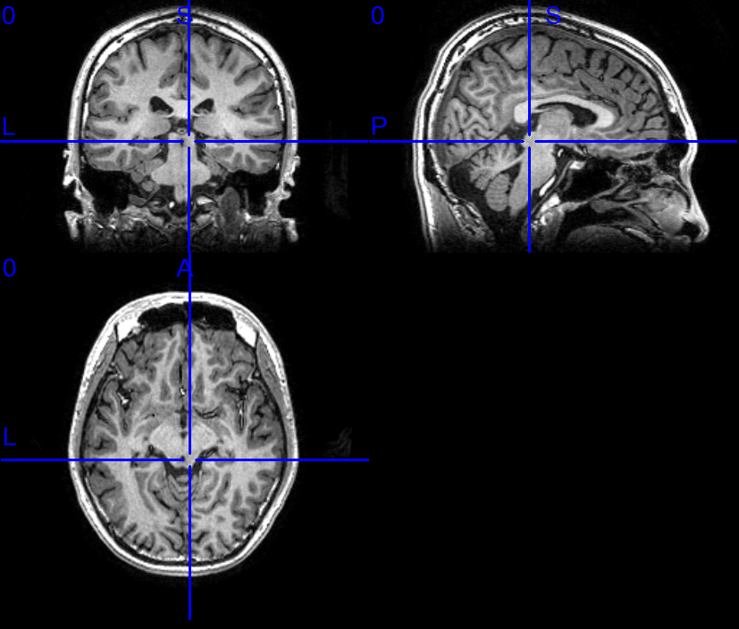
\includegraphics[width=0.5\linewidth]{figures/depression/sMRI.png}
	}
	%\\
	%\vspace{-2mm}
	\subfloat[fMRI images]{
		\label{fig_hard_case2}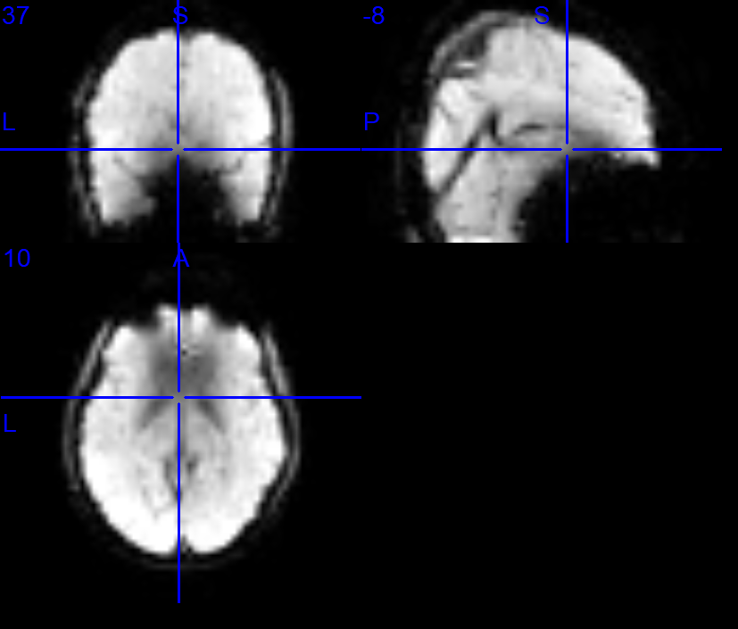
\includegraphics[width=0.5\linewidth]{figures/depression/fMRI.png}
	}
	
	\caption{
	Three View of MRI images~\cite{marek2011parkinson}.
	}
	\label{MRI}
\end{figure}

\subsubsection{Brain metabolic imaging}
%%%%%%%%%%%%%%%%%%%%%%%%%%%%%%%%%%%%%%%
Brain metabolic imaging provides an accurate understanding of nerve cell activity and metabolic changes under normal conditions and disease states, as well as the metabolic situation of the cerebral cortex under different physiological conditions of stimulation and thinking activity. Brain metabolic imaging such as PET and MRS can visualize the metabolic activity and various physiological or pathological metabolic changes in human brain and reflect them in the form of images.

PET uses the decay law or distribution characteristics of substances related to nuclear radiation, such as glucose, proteins, nucleic acids, etc., in the research object to obtain detailed information to reflect their metabolic activities to achieve the purpose of diagnosis.
PET is mainly based on the annihilation effect of positrons and electrons and can be used to explore characteristic pathological states and indicators in depressed patients. By investigating the correlation between changes in metabolic function in MDD brain regions and depressive symptoms, it was found that compared to normal healthy subjects, depressed patients usually show such phenomena as decreased regional cerebral blood flow values and standardized glucose uptake values in the prefrontal lobe, increased total distribution of translocated proteins, and increased inflammatory markers~\cite{2017Functional,2017Elevated,li2018microglial,2014Cerebral}.

MRS uses nuclear chemical shifts to study molecular structure and can be used to detect metabolite concentrations in brain regions.
MRS can detect biochemical changes in the injured tissue of the body by magnetic resonance hydrogen spectroscopy, which can effectively observe the metabolism of the injured area and has some clinical value for early diagnosis of the depression.
It was found that N-acetylaspartate (NAA) levels were significantly lower in the left hippocampus, glutamine and glutamate (Glx) levels were significantly increased in the right hippocampus, and choline complex (Cho) and creatine (Cr) levels were significantly higher in depressed patients compared to controls, and correlated with the severity of depression in patients~\cite{2018Early,20181H,2013}.


%\subsection{PET}
%\label{sec_fquality}
%%%%%%%%%%%%%%%%%%%%%%%%%%%%%%%%%%%%%%%
%PET uses the decay law or distribution characteristics of substances related to nuclear radiation, such as glucose, proteins, nucleic acids, etc., in the research object to obtain detailed information to reflect their metabolic activities to achieve the purpose of diagnosis.

%By examining the correlation between changes in cerebral blood perfusion and glucose metabolic function in the prefrontal lobe and depressive symptoms, Fu found that regional cerebral blood flow values and standardized glucose uptake values in the prefrontal lobe were reduced in depressed patients compared to normal healthy subjects~\cite{2017Functional}.
%Holmes believes that major depression is associated with elevated peripheral inflammatory markers. By comparing the utilization of transporters in the anterior cingulate cortex, frontal cortex, and insulation of patients with depression and healthy controls, the results found that transporter availability was significantly increased in glial cells of the anterior cingulate cortex during episodes in patients with MDD~\cite{2017Elevated}.
%Li explored the relationship between microglia-mediated processes and the pathophysiology of MDD by examining the distribution of  translocator protein total distribution volume $(TSPO \quad V_T)$, the results showed that the increased total distribution of translocated proteins was associated with decreased cognitive function in patients with MDD~\cite{li2018microglial}.

%\subsection{MRS}
%\label{sec_fquality}
%%%%%%%%%%%%%%%%%%%%%%%%%%%%%%%%%%%%%%%
%MRS uses nuclear chemical shifts to study molecular structure and can be used to detect metabolite concentrations in brain regions.

%N-acetyl aspartate(NAA) measures were interrogated through examining their relationship to previously documented ELS markers-cerebrospinal fluid (CSF) corticotropin -releasing factor (CRF) concentrations, hippocampal volume, body mass and behavioral timidity. Coplan's study found that compared with the control group, the NAA level in the left hippocampus of depression patients was significantly reduced, and the Glutamine and Glutamate(Glx) level in the right hippocampus was significantly increased~\cite{2018Early}.

%%%%%%%%%%%%%%%%%%%%%%%%%%%%%%%%%%%%%%
Brain imaging technology has revealed abnormalities in brain structure, brain function and brain metabolism in patients with depression, providing new ideas for early diagnosis and optimization of treatment plans.

\subsubsection{Performance Comparison}
%%%%%%%%%%%%%%%%%%%%%%%%%%%%%%%%%%%%%%%
Table \ref{tab3} shows a summary of the experimental results based on brain imaging to detect depression, including the source and name of the method, the input brain imaging modality, the data set used (- represents that the data used were collected by ourselves), and the evaluation criteria of the experimental results, including Accuracy, FScore Precision, Recall, Sensitivity, Specificity, and Area Under Curve (AUC).

SVM dominates the machine learning classifiers and usually achieves good results when compared with other classifiers. And deep learning algorithms usually achieve higher recognition accuracy than machine learning classifiers.

\begin{table*}
\centering
\caption{Experimental results based on brain imaging}
\label{tab3}
\begin{tabular}{l|l|l|l|lllllll}

\hline
\multicolumn{1}{c|}{\multirow{2}{*}{ID}} & \multicolumn{1}{c|}{\multirow{2}{*}{Method}}                         & \multicolumn{1}{c|}{\multirow{2}{*}{Brain imaging}} & \multicolumn{1}{c|}{\multirow{2}{*}{Dataset}} & \multicolumn{7}{c}{Classification}                                                                                                                                                                                            \\
\multicolumn{1}{c|}{}                    & \multicolumn{1}{c|}{}                                                & \multicolumn{1}{c|}{}                               & \multicolumn{1}{c|}{}                         & \multicolumn{1}{c}{Accuracy} & \multicolumn{1}{c}{F Score} & \multicolumn{1}{c}{Precision} & \multicolumn{1}{c}{Recall} & \multicolumn{1}{c}{Sensitivity} & \multicolumn{1}{c}{Specificity} & \multicolumn{1}{c}{AUC} \\
\hline
1                                       & SVM.~\cite{2015Automatic}           & fNIRS                                              & -                                            & 86.76                        & -                            & -                             & -                          & -                               & -                               & -                       \\
2                                       & RF+XGBoost~\cite{2020Classifying}           & fNIRS                                              & -                                            & 92.58                        & -                            & -                             & -                          & 84.78                           & 91.05                           & -                       \\
%3                                       & Chao et al.~\cite{2021fNIRS}                & fNIRS                                              & -                                            & 99.94                        & -                            & -                             & -                          & -                               & -                               & -                       \\
3                                       & AlexNet~\cite{2021Depression}                 & fNIRS                                              & -                                            & 90.00                        & -                            & 91.00                         & -                          & -                               & -                               & -                       \\
4                                       & ALSTMIT~\cite{ 2020DISTINGUISHING }           & fNIRS                                              & -                                            & 96.20                        & -                            & -                             & -                          & -                               & -                               & -                       \\
5                                       & SVM~\cite{2017Automatic}                      & fNIRS                                              & -                                            & 85.15                        & -                            & -                             & -                          & -                               & -                               & -                       \\
\hline
6                                       & CNN-LSTM~\cite{mousavian2020depression}      & RS-fMRI                                            & NKI online dataset                           & 100.00                       & -                            & -                             & -                          & 86.00                           & 0.00                            & 50.00                   \\
7                                       & ST-CNN~\cite{mousavian2020depression}        & RS-fMRI                                            & NKI online dataset                           & 100.00                       & -                            & -                             & -                          & 86.00                           & 0.00                            & 50.00                   \\
8                                       & 3D CNN~\cite{mousavian2020depression}        & RS-fMRI                                            & NKI online dataset                           & 90.00                        & -                            & -                             & -                          & 79.00                           & 10.00                           & 50.00                   \\
9                                       & 3D VGG-16~\cite{mousavian2020depression}     & RS-fMRI                                            & NKI online dataset                           & 100.00                       & -                            & -                             & -                          & 86.00                           & 0.00                            & 50.00                   \\
10                                       & FCN~\cite{mousavian2020depression}           & RS-fMRI                                            & NKI online dataset                           & 94.00                        & -                            & -                             & -                          & 79.00                           & 96.00                           & 88.00                   \\
11                                      & FCN\_woT-test~\cite{mousavian2020depression} & RS-fMRI                                            & NKI online dataset                           & 86.00                        & -                            & -                             & -                          & 0.00                            & 100.00                          & 50.00                   \\
12                                      & FCN\_CanICA~\cite{mousavian2020depression}   & RS-fMRI                                            & NKI online dataset                           & 87.00                        & -                            & -                             & -                          & 70.00                           & 90.00                           & 80.00                   \\
13                                      & DCF+SVM~\cite{2020Quantitative}            & RS-fMRI                                            & -                                            & 95.59                        & -                            & -                             & -                          & 96.77                           & 94.68                           & 99.13                   \\
14                                      & SVM~\cite{2016Multivariate}               & RS-fMRI                                            & -                                            & 76.10                        & -                            & -                             & -                          & 81.50                           & 68.90                           & -                       \\
15                                      & Unsupervised ML~\cite{2014Unsupervised}         & RS-fMRI                                            & -                                            & 92.50                        & -                            & -                             & -                          & -                               & -                               & -                       \\
16                                      & FCN+GAN~\cite{2020Functional}           & RS-fMRI                                            & -                                            & 70.10                        & 70.30                        & -                             & -                          & 73.50                           & 66.50                           & 70.30                   \\
17                                      & SVM~\cite{2013Identifying}             & RS-fMRI                                            & -                                            & 90.00                        & -                            & -                             & -                          & -                               & -                               & -                       \\
18                                     & GAN~\cite{2020Functional}                     & RS-fMRI                                            & -                                            & 80.70                        & -                            & -                             & -                          & -                               & -                               & -                       \\
19                                      & GCNs~\cite{2020Identifying}                   & RS-fMRI                                            & -                                            & 74.10                        & -                            & -                             & -                          & 56.60/46.6                      & 86.90                           & 79.10                   \\
20                                      &SVM-FoBa~\cite{Nan-Feng}                  & RS-fMRI                                            & -                                            & 84.78                        & 83.72                        & 91.30                         & 78.26                      & -                               & -                               & -                       \\
21                                     & MVPA~\cite{8575800}                    & RS-fMRI                                            & -                                            & 90.22                        & 89.89                        & 93.02                         & 86.96                      & -                               & -                               & -                       \\
22                                      & LASSO~\cite{ 2020Generalizable} & RS-fMRI                                               & -                                            & 70.00                        & -                            & -                             & -                          & -                               & -                               & -    \\
\hline
%22                                      & Gui et al.~\cite{2019The1}                  & TS-fMRI                                            & -                                            & 94.68                        & 94.38                        & -                             & 89.36                      & -                               & -                               & 98.87                   \\
%23                                      & Gui et al.~\cite{2019The1}                    & TS-fMRI                                            & -                                            & 94.68                        & 94.38                        & -                             & 89.36                      & -                               & -                               & 98.87                   \\
%24                                      & KNN~\cite{2019The1}                           & TS-fMRI                                            & --                                           & 52.13                        & 38.36                        & -                             & 29.79                      & -                               & -                               & 54.30                   \\
%25                                      & SVM~\cite{2019The1}                           & TS-fMRI                                            & -                                            & 79.79                        & 79.12                        & -                             & 76.60                      & -                               & -                               & 89.18                   \\
%26                                      & LR~\cite{2019The1}                            & TS-fMRI                                            & -                                            & 78.72                        & 76.74                        & -                             & 70.21                      & -                               & -                               & 86.28                   \\
%27                                      & DNN~\cite{2019The1}                           & TS-fMRI                                            & -                                            & 91.49                        & 91.30                        & -                             & 89.36                      & -                               & -                               & 97.01                   \\
%28                                      & GoogleNet~\cite{2019The1}                     & TS-fMRI                                            & -                                            & 86.17                        & 85.39                        & -                             & 80.85                      & -                               & -                               & 93.93                   \\
   
%\hline
23                                      & sLASSO~\cite{2015Toward}                      & fMRI                                               & -                                            & 83.82                        & 84.00                        & -                             & -                          & 84.61                           & 83.03                           & -                       \\
24                                      & gLASSO~\cite{2015Toward}                      & fMRI                                               & -                                            & 91.95                        & 92.00                        & -                             & -                          & 91.35                           & 92.55                           & -                       \\
25                                     & sgLASSO~\cite{2015Toward}                     & fMRI                                               & -                                            & 90.08                        & 90.00                        & -                             & -                          & 88.45                           & 91.73                           & -                       \\
\hline 
\end{tabular}
\end{table*}

%MVPA (Multivariate pattern analysis)

\ifx\allfiles\undefined
% !TEX root = tnnls_relation_gait.tex

% if have a single appendix:
%\appendix[Proof of the Zonklar Equations]
% or
%\appendix  % for no appendix heading
% do not use \section anymore after \appendix, only \section*
% is possibly needed

% use appendices with more than one appendix
% then use \section to start each appendix
% you must declare a \section before using any
% \subsection or using \label (\appendices by itself
% starts a section numbered zero.)
%

%\appendices
%\section{Proof of the First Zonklar Equation}
%Appendix one text goes here.
%
%% you can choose not to have a title for an appendix
%% if you want by leaving the argument blank
%\section{}
%Appendix two text goes here.

% use section* for acknowledgment
% \section*{Acknowledgment}
% The authors would like to thank Prof. Dongbin Zhao for his support to this work.

% Can use something like this to put references on a page
% by themselves when using endfloat and the captionsoff option.
\ifCLASSOPTIONcaptionsoff
  \newpage
\fi

% trigger a \newpage just before the given reference
% number - used to balance the columns on the last page
% adjust value as needed - may need to be readjusted if
% the document is modified later
%\IEEEtriggeratref{8}
% The "triggered" command can be changed if desired:
%\IEEEtriggercmd{\enlargethispage{-5in}}

% references section

% can use a bibliography generated by BibTeX as a .bbl file
% BibTeX documentation can be easily obtained at:
% http://mirror.ctan.org/biblio/bibtex/contrib/doc/
% The IEEEtran BibTeX style support page is at:
% http://www.michaelshell.org/tex/ieeetran/bibtex/
\bibliographystyle{IEEEtran}
% argument is your BibTeX string definitions and bibliography database(s)
\bibliography{IEEEabrv,tnnls_relation_gait}
%
% <OR> manually copy in the resultant .bbl file
% set second argument of \begin to the number of references
% (used to reserve space for the reference number labels box)
%\begin{thebibliography}{1}
%\bibitem{IEEEhowto:kopka}
%H.~Kopka and P.~W. Daly, \emph{A Guide to \LaTeX}, 3rd~ed.\hskip 1em plus
%  0.5em minus 0.4em\relax Harlow, England: Addison-Wesley, 1999.
%\end{thebibliography}

% biography section
%
% If you have an EPS/PDF photo (graphicx package needed) extra braces are
% needed around the contents of the optional argument to biography to prevent
% the LaTeX parser from getting confused when it sees the complicated
% \includegraphics command within an optional argument. (You could create
% your own custom macro containing the \includegraphics command to make things
% simpler here.)
%\begin{IEEEbiography}[{\includegraphics[width=1in,height=1.25in,clip,keepaspectratio]{mshell}}]{Michael Shell}
% or if you just want to reserve a space for a photo:

%\begin{IEEEbiography}{Michael Shell}
%Biography text here.
%\end{IEEEbiography}
%
%% if you will not have a photo at all:
%\begin{IEEEbiographynophoto}{John Doe}
%Biography text here.
%\end{IEEEbiographynophoto}

% insert where needed to balance the two columns on the last page with
% biographies
% \newpage

%\begin{IEEEbiographynophoto}{Jane Doe}
%Biography text here.
%\end{IEEEbiographynophoto}

%\begin{IEEEbiography}[{\includegraphics[width=1in,height=1.25in,clip,keepaspectratio]{photos/hsh.pdf}}]{Saihui Hou}
%% \begin{IEEEbiographynophoto}{Saihui Hou}
%	received the B.E. and Ph.D. degrees from University of Science and Technology of China in 2014 and 2019, respectively.
%    %
%    He is currently an Assistant Professor with School of Artificial Intelligence, Beijing Normal University.
%    %
%    His research interests include computer vision and machine learning.
%    %
%    He focuses on gait recognition which aims to identify different people according to the walking patterns.
%% \end{IEEEbiographynophoto}
%\end{IEEEbiography}
%
%\begin{IEEEbiography}[{\includegraphics[width=1in,height=1.25in,clip,keepaspectratio]{photos/lx.pdf}}]{Xu Liu}
%% \begin{IEEEbiographynophoto}{Xu Liu}
%	received the B.E. and Ph.D. degrees from University of Science and Technology of China in 2013 and 2018, respectively.
%    %
%    He is currently a Research Scientist with Watrix Technology Limited Co. Ltd.
%    %
%    His research interests include gait recognition, object detection and image segmentation.
%% \end{IEEEbiographynophoto}
%\end{IEEEbiography}
%
%\begin{IEEEbiography}[{\includegraphics[width=1in,height=1.25in,clip,keepaspectratio]{photos/ccs.pdf}}]{Chunshui Cao}
%% \begin{IEEEbiographynophoto}{Chunshui Cao}
%	received the B.E. and Ph.D. degrees from University of Science and Technology of China in 2013 and 2018, respectively.
%    %
%    During his Ph.D. study, he joined Center for Research on Intelligent Perception and Computing, National Laboratory of Pattern Recognition, Institute of Automation, Chinese Academy of Sciences.
%    %
%    From 2018 to 2020, he worked as a Postdoctoral Fellow with PBC School of Finance, Tsinghua University.
%    %
%    He is currently a Research Scientist with Watrix Technology Limited Co. Ltd.
%    %
%    His research interests include pattern recognition, computer vision and machine learning.
%% \end{IEEEbiographynophoto}
%\end{IEEEbiography}
%
%\begin{IEEEbiography}[{\includegraphics[width=1in,height=1.25in,clip,keepaspectratio]{photos/hyz.pdf}}]{Yongzhen Huang}
%% \begin{IEEEbiographynophoto}{Yongzhen Huang}
%	received the B.E. degree from Huazhong University of Science and Technology in 2006, and the Ph.D. degree from Institute of Automation, Chinese Academy of Sciences in 2011.
%    %
%    He is currently an Associate Professor with School of Artificial Intelligence, Beijing Normal University.
%    %
%    He has published one book and more than 80 papers at international journals and conferences such as TPAMI, IJCV, TIP, TSMCB, TMM, TCSVT, CVPR, ICCV, ECCV, NIPS, AAAI.
%    %
%    His research interests include pattern recognition, computer vision and machine learning.
%% \end{IEEEbiographynophoto}
%\end{IEEEbiography}


\end{document}

\fi 